\documentclass{article}

\usepackage[margin=3cm]{geometry}

\geometry{a4paper,left=2cm,right=2cm,top=2.54cm,bottom=2.54cm}
%加這個就可以設定字體
\usepackage{fontspec}
    % 普通文字,行距
        \usepackage[onehalfspacing]{setspace}
    
    % 段落間距  (begin doc 才設定)
        \usepackage{parskip}
%使用xeCJK,其他的還有CJK或是xCJK
    % 中文
    \usepackage{xeCJK}
    \setCJKmainfont[AutoFakeBold=3]{DFKai-SB} %设置中
    \usepackage[fontsize=14pt]{fontsize}
% 首行縮排距離
    \setlength\parindent{28pt}
        % 首行縮排
        \usepackage{indentfirst}

%%%%%%%%%%%%%%%%%%%%%%%%
%%%%    三、圖片
%%%%%%%%%%%%%%%%%%%%%%%%


    %%%%    啟用圖片功能
    \usepackage{graphicx}

    %%%%    設定圖片路徑
    \graphicspath{ {./img/} }

    %%%%    設定圖片定位
    \usepackage{float}

    %%%%    把Figure變成"圖"
    \renewcommand{\figurename}{Fig}

%%%%%%%%%%%%%%%%%%%%%%%%
%%%%%%%              end

% 目錄顯示層次
    \setcounter{tocdepth}{2}
% 計算
\usepackage{enumitem}

%設定英文字型,不設的話就會使用預設的字型
\setmainfont{Times New Roman}

\usepackage{fontspec}
\usepackage{titlesec}
\usepackage{graphicx}
\usepackage{physics}
\usepackage{amsmath}
\usepackage{mathtools}
\usepackage{setspace}
\usepackage{subfigure} %所需宏包

\usepackage[hidelinks]{hyperref}
 \usepackage{titlesec}
    % 定义section格式,包括中文数字
   
    \usepackage{zhnumber}
\titleformat{\section}
  {\fontsize{18pt}{15}\bfseries}
  {\selectfont\thesection.}
  {0.5em}
  {}

\usepackage{fancyhdr}
\pagestyle{fancy}

\usepackage{color, xcolor}

\usepackage{algorithm}
\usepackage{algpseudocode}


% New definitions
\algnewcommand\algorithmicswitch{\textbf{switch}}
\algnewcommand\algorithmiccase{\textbf{case}}
\algnewcommand\algorithmicassert{\texttt{assert}}
\algnewcommand\Assert[1]{\State \algorithmicassert(#1)}%
% New "environments"
\algdef{SE}[SWITCH]{Switch}{EndSwitch}[1]{\algorithmicswitch\ #1\ \algorithmicdo}{\algorithmicend\ \algorithmicswitch}%
\algdef{SE}[CASE]{Case}{EndCase}[1]{\algorithmiccase\ #1}{\algorithmicend\ \algorithmiccase}%
\algtext*{EndSwitch}%
\algtext*{EndCase}%

\usepackage{newfloat}
\DeclareFloatingEnvironment[
  fileext = lol ,
  listname = {List Of Listings} ,
  name = Listing
]{listing}

\makeatletter
\newenvironment{breakablealgorithm}
  {% \begin{breakablealgorithm}
    \footnotesize
   \begin{center}
     \refstepcounter{algorithm}% New algorithm
     \hrule height.8pt depth0pt \kern2pt% \@fs@pre for \@fs@ruled
     \renewcommand{\caption}[2][\relax]{% Make a new \caption
       {\raggedright\textbf{\ALG@name~\thealgorithm} ##2\par}%
       \ifx\relax##1\relax % #1 is \relax
         \addcontentsline{loa}{algorithm}{\protect\numberline{\thealgorithm}##2}%
       \else % #1 is not \relax
         \addcontentsline{loa}{algorithm}{\protect\numberline{\thealgorithm}##1}%
       \fi
       \kern2pt\hrule\kern2pt
     }
  }{% \end{breakablealgorithm}
     \kern2pt\hrule\relax% \@fs@post for \@fs@ruled
   \end{center}
  }
\makeatother

\usepackage{pdfpages}
\algnewcommand\And{\textbf{and}}
\algnewcommand\Or{\textbf{or}}

\usepackage{amsmath}

\newcommand\mycommfont[1]{\footnotesize\ttfamily\textcolor{mygreen}{#1}}

\usepackage{tikz, ifthen}
\usetikzlibrary{calc,shapes, positioning,chains,arrows}

\usepackage{everyshi}  % 用于在每一页应用浮水印


% 畫底線
\usepackage{ulem}


\definecolor{myblue}{HTML}{6B73D5}
\definecolor{myred}{HTML}{C00000}
\definecolor{myyellow}{HTML}{FFDB57}

\usepackage[hidelinks]{hyperref}
\hypersetup{urlcolor=myblue, % url
citecolor=black, % citation
linkcolor=black, % table of contents, inner color
colorlinks=true, }
\usepackage{enumitem}

\usepackage{listings}

\definecolor{Blue}{rgb}{0,0,1}
\definecolor{Green}{rgb}{0,0.5,0}
\definecolor{Red}{rgb}{0.64,0.08,0.08}


\lstset{
    captionpos=t,                       % 讓Caption在Bottom的位置
    numbers=left,                       % 程式碼行號
    frame=single,
    showstringspaces=false,             % "不"標註空格
    escapeinside={(*@}{@*)},            % 脫逃字元
    commentstyle=\color{Green},         % Comment顏色
    keywordstyle=\color{Blue},          % Keyword顏色
    stringstyle=\color{Red},            % String顏色
    basicstyle=\ttfamily\scriptsize,         % 字型
    breaklines = true,
}


\begin{document}



\thispagestyle{empty}

\begin{center}
        \vspace*{3cm} %垂直距離
        {\Huge\bf
            \underline{CAD for VLSI Design }\\}%\uppercase\expandafter{\romannumeral 1}}
        \vspace{3cm}
        {\bf\huge Project Assignment 4\\}
        \vspace{0.5cm}
        {\bf\fontsize{23pt}{20}\selectfont IR-drop Prediction\\}
        \vspace{4cm}
        {\fontsize{23pt}{26pt} \selectfont Instructor: Andy, Yu-Guang Chen  Ph.D.\\}
        {\fontsize{20pt}{26pt} \selectfont TA: 蔡書儀\\}
        \vspace{2cm}
        \fontsize{22pt}{25pt}\selectfont
        Department/Class: Electrical Engineering 4A\\
        \vspace*{1em}
        Name: {\bf 陳緯亭}\\
        \vspace*{1em}
        Student ID Number: {\bf 109501201}\\
\vspace{2cm}
\end{center}
\newpage


\tableofcontents
\listoflistings


\thispagestyle{empty}
\newpage


 \setcounter{page}{1}

 \lhead{109501201\ 陳緯亭}

% --------------------------------------------------------


\section{The selection of training and validation sets.}

The data was selected at random. With regard to the training set, 70 datasets were randomly selected. With regard to the validation set, 10 datasets were randomly selected. The objective is to perturb the datasets.

\begin{figure}[H]
    \centering
    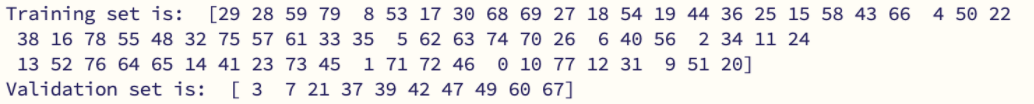
\includegraphics[width=\linewidth]{./img/2024-06-13-22-32-17.png}
    \caption{The selection of training and validation sets}
    \label{sel}
  \end{figure}

\section{The feature selections and parameter settings}

The feature was selected based on the model feature importances. The scores for MSE, RMSE, MAE, and CC were observed in order to determine which features were to be retained. The least important feature should be retained or deleted based on an assessment of its relative importance. The code can be observed in [Listing~\ref{sort}], and the result can be found in Figs~[\ref{f1}] and [\ref{f2}].

\begin{figure}[H]
    \centering
\includegraphics*[width=0.4\linewidth]{./img/2024-06-13-22-29-38.png}
\caption{Features sort by importance}
\label{f1}
\end{figure}

\begin{figure}[H]
    \centering
\includegraphics*[width=0.9\linewidth]{/Users/chenweiting/Documents/GitHub/NOW/CAD/PA4/PA4_SampleCode/feature_importance.png}
\caption{Features sort by importance}
\label{f2}
\end{figure}


\begin{lstlisting}[language={python}, caption={Features sort by importance}, label={sort}]
    import xgboost as xgb
    from sklearn.model_selection import train_test_split
    import pandas as pd
    import numpy as np
    import matplotlib.pyplot as plt
    import os
    import random
    
    # Define file path and filename
    DataSet_Path = "/home/CAD112/PA4/Training/"
    for i in range(1, 21):
        index = random.sample(range(1, 79), 1)[0]
        files = [f"MEMC_{index}.csv"] 
        print(f"MEMC_{index}.csv loaded...")
    
    # Extract features and labels
    selected_features = ['y', 'SPR', 'Reff', 'x', 'Tarrival', 'TCinternal', 'w', 'Cell type', 'Pinternal', 'Pleak', 'Ipeak', 'Ttransition', 'Cload']
    all_data = []
    
    # Read and combine data
    for file in files:
        data = pd.read_csv(os.path.join(DataSet_Path, file))
        all_data.append(data)
    
    # Combine all data
    combined_data = pd.concat(all_data)
    
    # Extract features and labels
    X = combined_data[selected_features]
    y = combined_data["IR-drop"]
    
    # Split into training and testing sets
    X_train, X_test, y_train, y_test = train_test_split(X, y, test_size=0.2, random_state=9527)
    
    # Train the model
    model = xgb.XGBRegressor(objective='reg:squarederror')
    model.fit(X_train, y_train)
    
    # Get feature importance
    importance = model.feature_importances_
    importance_df = pd.DataFrame({
        'Feature': selected_features,
        'Importance': importance
    })
    
    # Sort by importance
    importance_df = importance_df.sort_values(by='Importance', ascending=False)
    print(importance_df)
    
    # Predict and calculate scores
    y_train_pred = model.predict(X_train)
    y_test_pred = model.predict(X_test)
    
    def score(y_true, y_pred):
        mse = np.mean((y_true - y_pred) ** 2)
        rmse = np.sqrt(mse)
        mae = np.mean(np.abs(y_true - y_pred))
        cc = np.corrcoef(y_true, y_pred)[0, 1]
        return mse, rmse, mae, cc
    
    train_mse, train_rmse, train_mae, train_cc = score(y_train, y_train_pred)
    test_mse, test_rmse, test_mae, test_cc = score(y_test, y_test_pred)
    
    print('Train MSE:', train_mse)
    print('Train RMSE:', train_rmse)
    print('Train MAE:', train_mae)
    print('Train CC:', train_cc)
    
    print('Test MSE:', test_mse)
    print('Test RMSE:', test_rmse)
    print('Test MAE:', test_mae)
    print('Test CC:', test_cc)
    
    # Visualize feature importance
    plt.figure(figsize=(10, 6))
    plt.barh(importance_df['Feature'], importance_df['Importance'])
    plt.xlabel('Importance')
    plt.ylabel('Feature')
    plt.title('Feature Importance')
    plt.gca().invert_yaxis()
    
    # Save the image
    plt.savefig('feature_importance.png', bbox_inches='tight')
    plt.show()
    \end{lstlisting}


  In order to ascertain the optimal configuration, I employed the methodology outlined in [Listing~\ref{sort}]. Through a process of trial and error, I identified the following features as the most suitable for the given context. The outcome of this process is illustrated in Fig~[\ref{pf}]. [Listing~\ref{lf}]

  \begin{figure}[H]
    \centering
    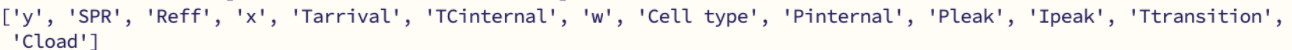
\includegraphics[width=\linewidth]{./img/2024-06-13-22-33-47.png}
    \caption{The selection of training and validation sets}
    \label{pf}
  \end{figure}

  \vspace*{-1em} 

\begin{lstlisting}[language={python}, caption={Get features}, label={lf}]
# Get all input feature
def get_feature():
    # ******************************************************************
    # TODO 2: Select the features for training
    # Sample: feature_name = ["x", "y", "w", "h"]
    # Note that you should not put "IR-drop" as your training features
    
    feature_name = ['y','SPR','Reff','x','Tarrival','TCinternal','w','Cell type','Pinternal','Pleak','Ipeak','Ttransition','Cload'] 
    print(feature_name)
    np.save("./feature_name.npy",np.array(feature_name))
    # END of TODO 2
    # ******************************************************************    
\end{lstlisting}

In order to define the model parameters, a series of trials were conducted, with the results recorded at each stage. This process was repeated until the desired outcome was achieved. Furthermore, it was observed that certain parameters had no impact on the results. For instance, the parameters "subsample," "colsample\_bytree," "colsample\_bylevel," "colsample\_bynode," "gamma," and so forth. Consequently, these parameters were set to their default values. [Listing~\ref{lp}]

\begin{lstlisting}[language={python}, caption={Define model parameters}, label={lp}]
# ******************************************************************
# TODO 3: Define model parameters
# You can add more parameter settings if needed

param = {
    'max_depth': 8,  # Maximum depth of the tree
    'eta': 0.4,  # Learning rate
    'eval_metric': "rmse",  # Evaluation metric
    'objective': "reg:squarederror",  # Objective function
    'lambda': 1,  # L2 regularization
    'n_estimators': 500,  # Number of trees
    # 'subsample': 0.8,  # Subsample ratio
    # 'colsample_bytree': 0.8,  # Feature ratio per tree
    # 'colsample_bylevel': 0.8,  # Feature ratio per level
    # 'colsample_bynode': 0.8,  # Feature ratio per node
    # 'gamma': 0.1,  # Minimum loss reduction
    # 'min_child_weight': 1,  # Minimum sum of instance weight
    # 'alpha': 0.1  # L1 regularization
}
# END of TODO 3
# ******************************************************************
\end{lstlisting}

Following a comprehensive investigation, it was established that the optimal training iteration was 30. Consequently, the value of num\_round was set to 50 in order to ensure a greater degree of possibility. [Listing~\ref{li}]

\begin{lstlisting}[language={python}, caption={Determine training itreation}, label={li}]
# TODO 4: Determine training itreation
num_round = 50
\end{lstlisting}

Furthermore, the early stopping rounds were adjusted in order to prevent overfitting during the training process. Fig~[\ref{stop}]

\begin{figure}[H]
    \centering
    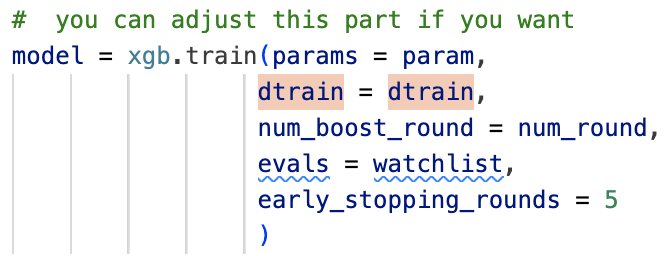
\includegraphics[width=0.5\linewidth]{./img/2024-06-13-23-06-01.png
    }
    \caption{Early stopping rounds}
    \label{stop}
  \end{figure}

\section{ The evaluation results}

\begin{figure}[H]
    \centering
    \includegraphics[width=0.5\linewidth]{/Users/chenweiting/Downloads/2024-06-13-21-59-55-image.png}
    \caption{The evaluation result}
    \label{ans}
  \end{figure}


\section{The hardness of this assignment / I overcome it}

\begin{enumerate}

\item What are the distinctions between objective and evaluative metrics?\\ 
The objective is to optimise the model. Evaluative metrics are employed to assess the model's effectiveness. Consequently, evaluative metrics exert no influence on the training of the model.
\href{https://reurl.cc/nNR4Ge}{xgboost objective和eval\_metric的區別}


\item What parameters can be modified? \\
\href{https://blog.csdn.net/wwlsm_zql/article/details/126192959}{XGB系列-XGB参数指南}

\item Whether the tree\_method can utilise gpu\_hist.\\
The output would be "WARNING: /src/learner.cc:248: No visible GPU is found, setting `gpu\_id` to -1".

\end{enumerate}

% ------------------------------

\section{Bonus}


The results demonstrated that the outcome was inferior to that of XGBoost. It appears that the parameters and features must be modified according to the specific technology in question. Furthermore, the LightGBM algorithm generates the following warning message: "No further splits with positive gain were observed, with the best gain being -inf for every training." This is the primary reason for the unsatisfactory results. If you're looking for more information, you can find it in [Listing~\ref{sa}], [Listing~\ref{c1}], [Listing~\ref{c2}], and [Listing~\ref{c3}].

\begin{figure}[H]
    \centering
\includegraphics*[width=0.5\linewidth]{./img/2024-06-13-20-25-32.png}
\caption{The evaluation result of LightGBM}
\end{figure}

\lstinputlisting[caption={LightGBM\_Training}, label={sa}, language={python}]{/Users/chenweiting/Documents/GitHub/NOW/CAD/PA4/PA4_SampleCode/Training_gbm.py}

To evaluate the LightGBM, I have to modify the following three lines.

\begin{lstlisting}[language={python}, caption={LightGBM\_Evaluation change 1}, label={c1}]
dpredict = lgb.Dataset(X, feature_name=feature_name)
\end{lstlisting}


\begin{lstlisting}[language={python}, caption={LightGBM\_Evaluation change 2}, label={c2}]
# Require trained model to use below options
TRAINED_MODEL = "./model/PA4_Model.cbm"
\end{lstlisting}

\begin{lstlisting}[language={python}, caption={LightGBM\_Evaluation change 3}, label={c3}]
# Load the model
model = lgb.Booster(model_file=TRAINED_MODEL)
\end{lstlisting}



% ------------------------------

\section{Suggestions}

No.


% ------------------------------

\end{document}